\section{GitFlow}
\subsection{¿Qué es GitFlow?}

\quad Gitflow es un diseño de flujo de trabajo Git que se publicó por primera vez y se hizo popular por \textit{Vincent Driessen} en \textit{nvie}. El flujo de trabajo de Gitflow define un modelo de ramificación estricto diseñado en torno al lanzamiento del proyecto. Esto proporciona un marco robusto para gestionar proyectos más grandes.\\

\quad Gitflow es ideal para proyectos que tienen un ciclo de lanzamiento programado, pues este flujo de trabajo no agrega nuevos conceptos o comandos más allá de lo que se requiere para el Flujo de trabajo de la rama de funciones, si no que asigna roles muy específicos a diferentes ramas y define cómo y cuándo deben interactuar. Además de las ramas de características, utiliza ramas individuales para preparar, mantener y grabar lanzamientos. Por supuesto, también puede aprovechar todos los beneficios del flujo de trabajo de Branch Branch: solicitudes de extracción, experimentos aislados y una colaboración más eficiente.\\ 

\subsection{¿Cómo funciona? \cite{GitKraken2} \cite{GitFlow}}

\subsubsection{Ramas Develop \& Master}

\quad En lugar de una sola rama, este flujo de trabajo usa dos ramas para registrar el historial del proyecto.\\ 

\quad La rama \textit{master} almacena el historial de lanzamiento oficial, y la rama \textit{develop} sirve como una rama de integración de características. También es conveniente etiquetar todos los commits en master con un número de versión.\\

\begin{figure}[htb]
	\centering
	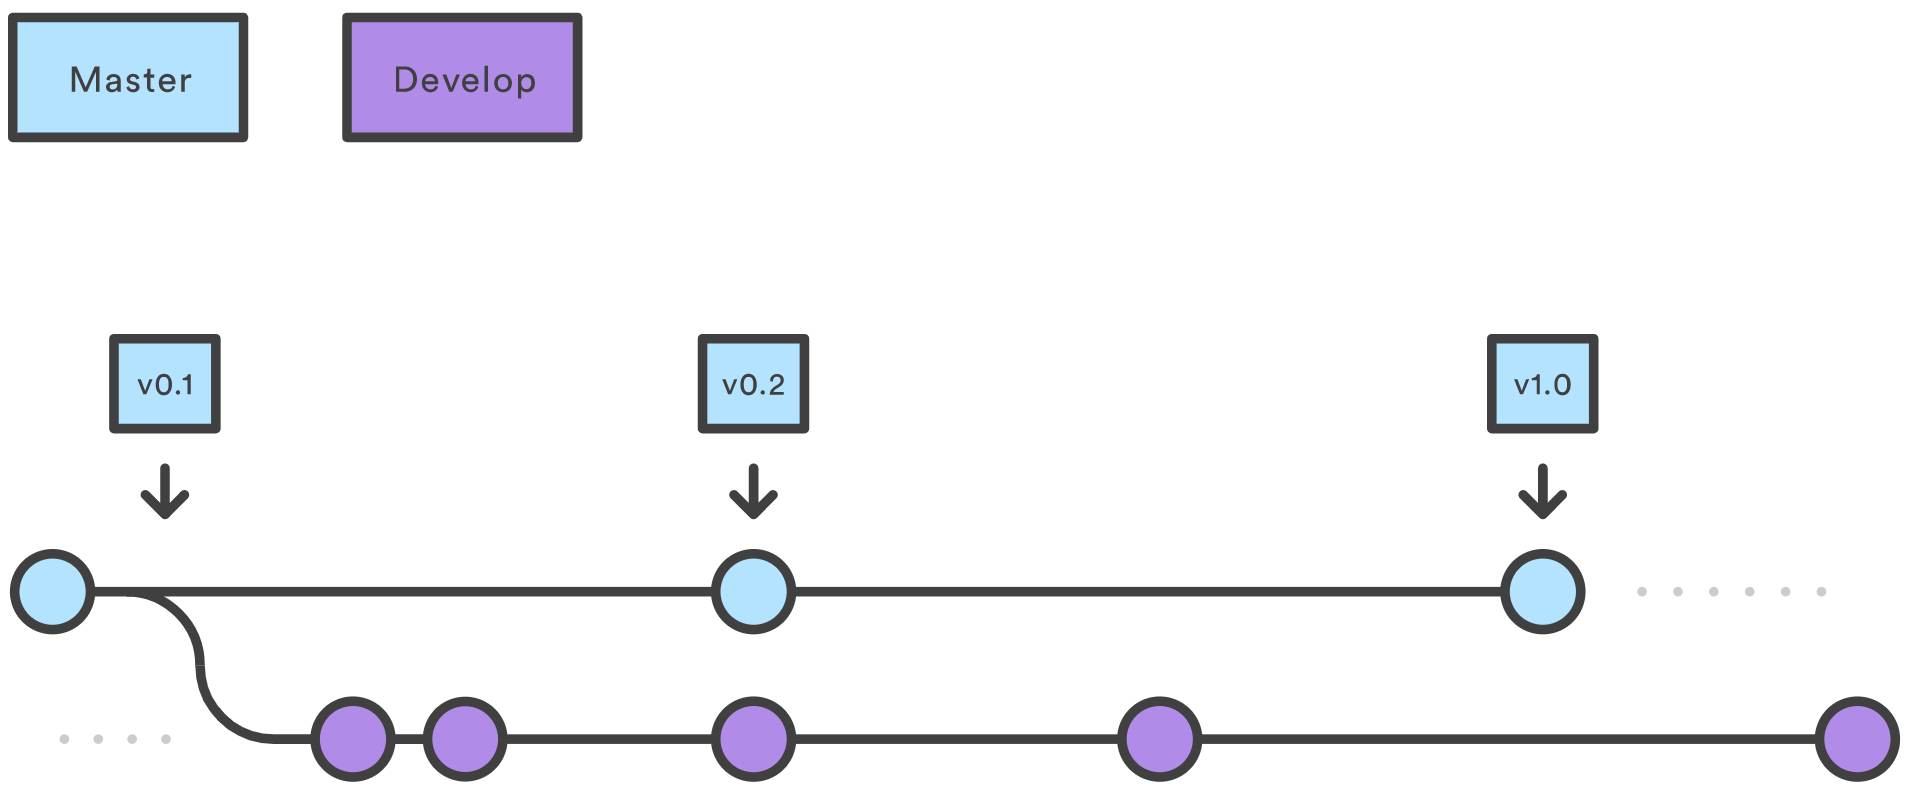
\includegraphics[width=0.75\textwidth]{./imagenes/master-dev}
	\caption{Ramas Develop y Master}
\end{figure}
\FloatBarrier

\subsubsection{Ramas Feature}

\quad Cada nueva feature debe residir en su propia rama, que se puede enviar al repositorio central como respaldo/colaboración.\\

\quad En lugar de bifurcarse de master, las features usan el desarrollo como su rama principal, de forma que cuando se completa una característica, se fusiona nuevamente en develop. Las características nunca deberían interactuar directamente con el maestro.\\

\begin{figure}[htb]
	\centering
	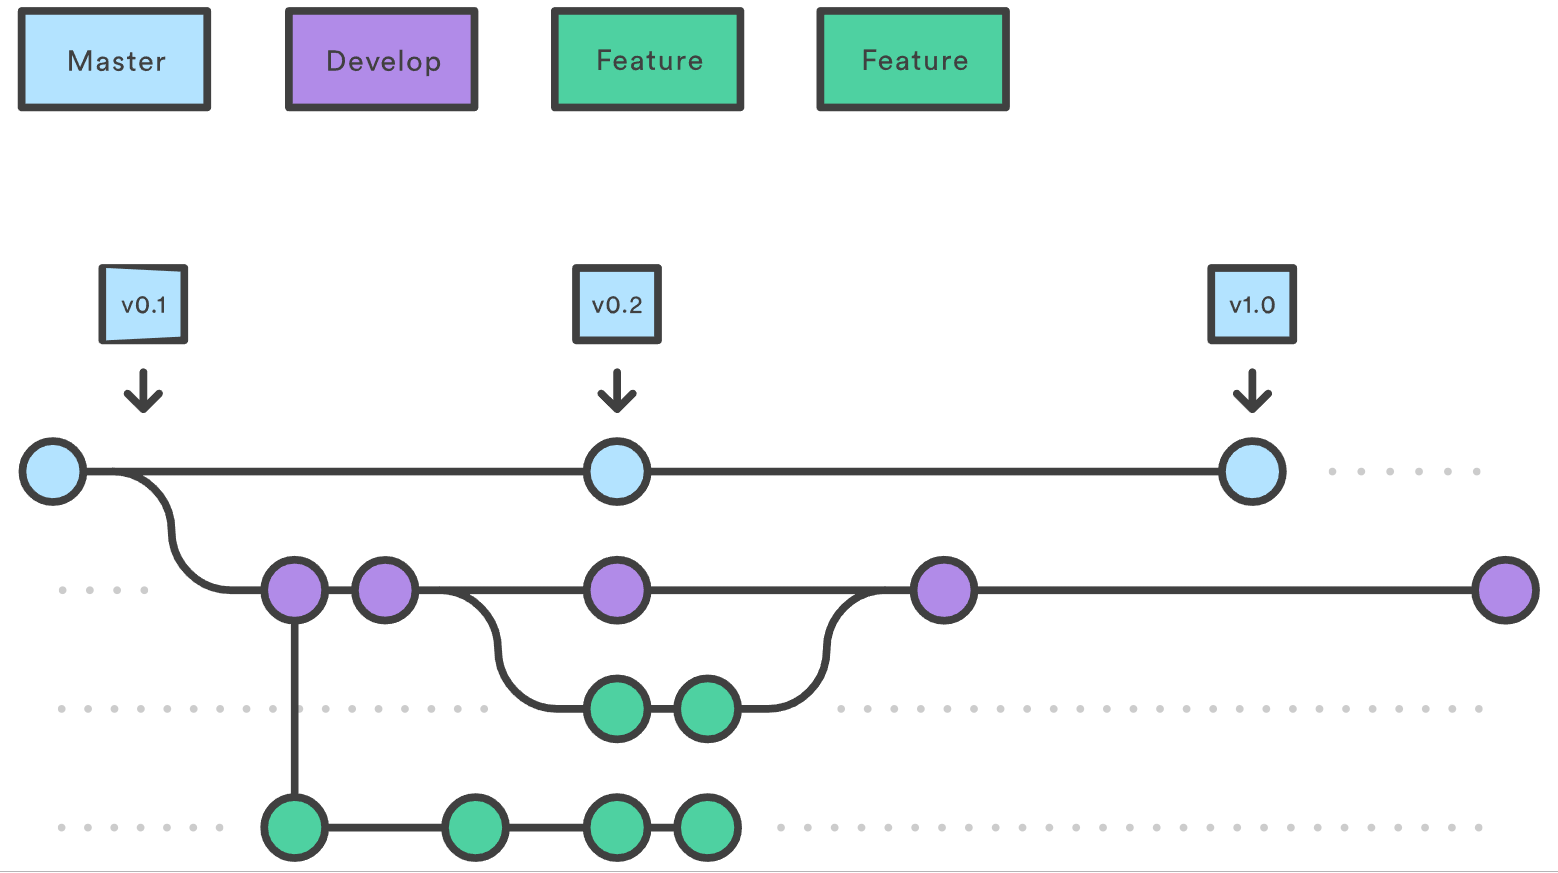
\includegraphics[width=1\textwidth]{./imagenes/feature}
	\caption{Rama feature}
\end{figure}
\FloatBarrier

\subsubsection{Ramas Release}

\quad Una vez que el desarrollo ha adquirido suficientes características para un lanzamiento,  bifurca una rama de release fuera del desarrollo. La creación de esta rama inicia el siguiente ciclo de lanzamiento, por lo que no se pueden agregar nuevas características después de este punto. Solo las correcciones de errores, la generación de documentación y otras tareas orientadas a la versión deben ir en esta rama.\\ 

\quad Una vez que está listo para enviar, la release se fusiona en master y se etiqueta con un número de versión. Además, debe fusionarse nuevamente en el desarrollo, que puede haber progresado desde que se inició el lanzamiento.\\

\begin{figure}[htb]
	\centering
	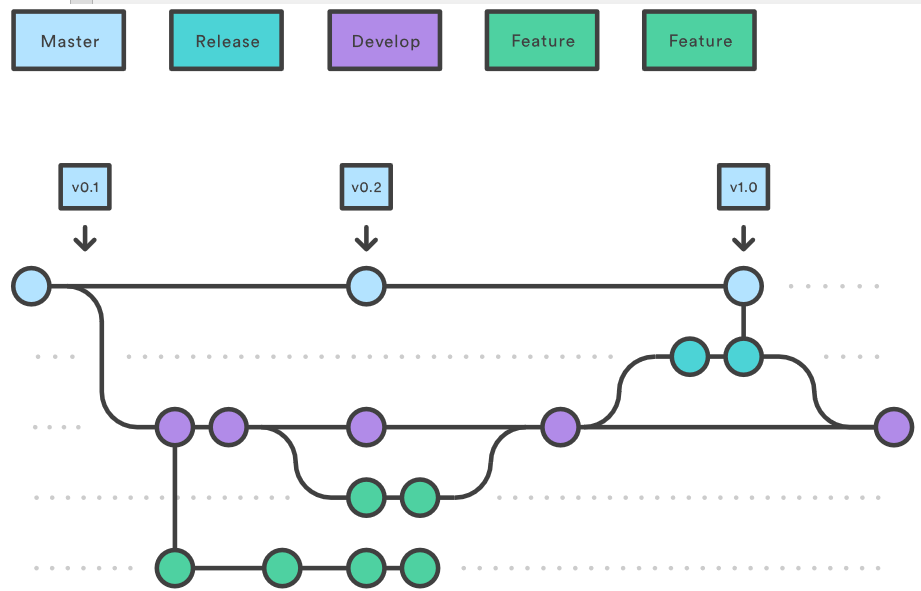
\includegraphics[width=1\textwidth]{./imagenes/release}
	\caption{Rama release}
\end{figure}
\FloatBarrier

\subsubsection{Ramas Hotfix}

\quad Las ramas de mantenimiento o "hotfix" se utilizan para parchear rápidamente las versiones de producción.\\

\quad Las ramificaciones de revisión son muy parecidas a las ramificaciones de lanzamiento y ramificaciones de características, excepto que se basan en master en lugar de develop.\\

\quad Esta es la única rama que debe bifurcarse directamente de master, y tan pronto como se complete la corrección, debe fusionarse tanto en master como en develop (o en la rama de la versión actual), y master debe etiquetarse con un número de versión actualizado.\\

\begin{figure}[htb]
	\centering
	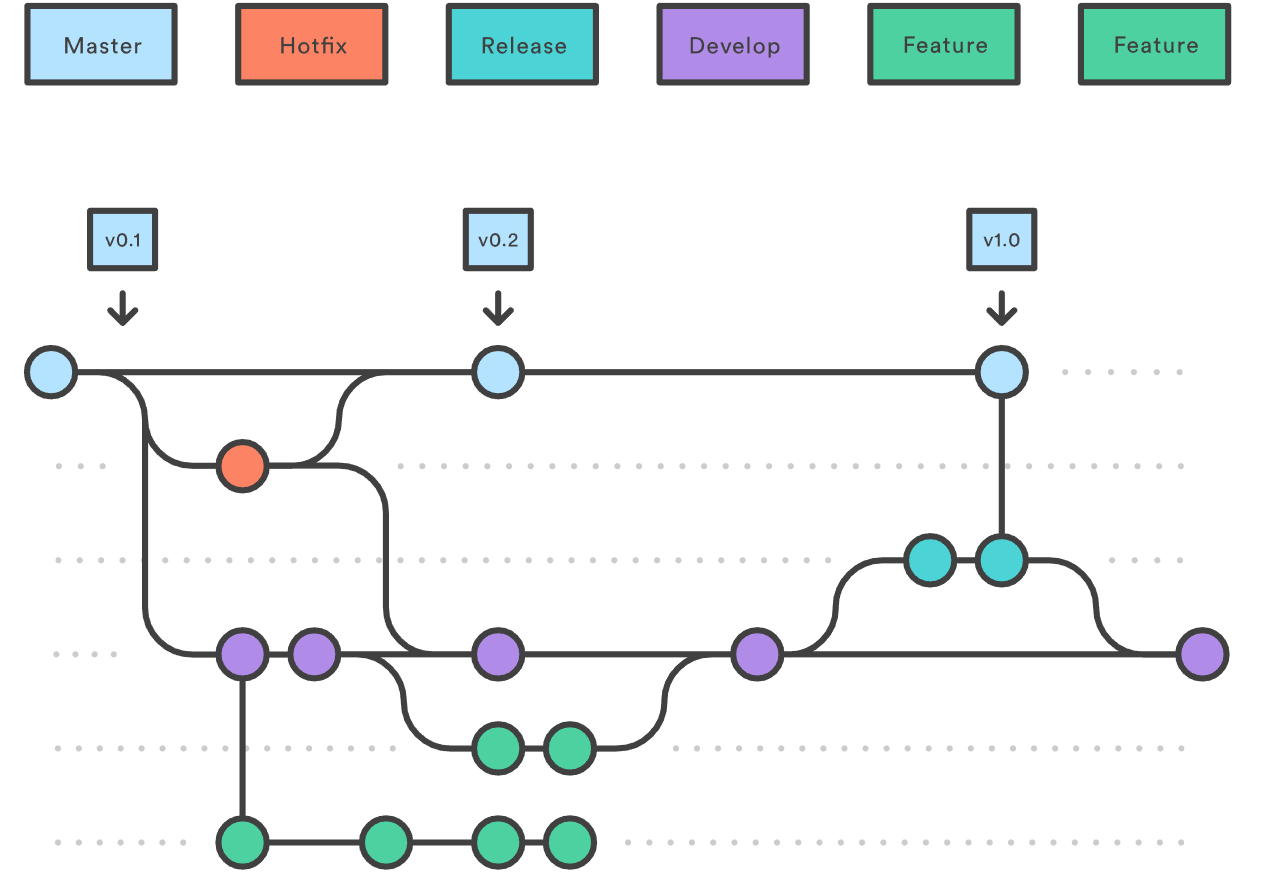
\includegraphics[width=0.6\textwidth]{./imagenes/hotfix}
	\caption{Rama hotfix}
\end{figure}
\FloatBarrier

\newpage
